%%%%%%%%%%%%%%%%%%%%%%%%%%%%%%%%%%%%%%%%%
% The Legrand Orange Book
% LaTeX Template
% Version 2.4 (26/09/2018)
%
% This template was downloaded from:
% http://www.LaTeXTemplates.com
%
% Original author:
% Mathias Legrand (legrand.mathias@gmail.com) with modifications by:
% Vel (vel@latextemplates.com)
%
% License:
% CC BY-NC-SA 3.0 (http://creativecommons.org/licenses/by-nc-sa/3.0/)
%
% Compiling this template:
% This template uses biber for its bibliography and makeindex for its index.
% When you first open the template, compile it from the command line with the 
% commands below to make sure your LaTeX distribution is configured correctly:
%
% 1) pdflatex main
% 2) makeindex main.idx -s StyleInd.ist
% 3) biber main
% 4) pdflatex main x 2
%
% After this, when you wish to update the bibliography/index use the appropriate
% command above and make sure to compile with pdflatex several times 
% afterwards to propagate your changes to the document.
%
% This template also uses a number of packages which may need to be
% updated to the newest versions for the template to compile. It is strongly
% recommended you update your LaTeX distribution if you have any
% compilation errors.
%
% Important note:
% Chapter heading images should have a 2:1 width:height ratio,
% e.g. 920px width and 460px height.
%
%%%%%%%%%%%%%%%%%%%%%%%%%%%%%%%%%%%%%%%%%

%----------------------------------------------------------------------------------------
%	PACKAGES AND OTHER DOCUMENT CONFIGURATIONS
%----------------------------------------------------------------------------------------

\documentclass[11pt,fleqn,dvipsnames]{book} % Default font size and left-justified equations
\usepackage[dvipsnames]{xcolor}
\usepackage{tikz}
\usepackage{graphicx}
\usetikzlibrary{arrows,automata,positioning,trees,shadows}

\usepackage[font=small]{caption}
\usepackage{listings}
\usepackage{clrscode3e}
\usepackage[final]{pdfpages}
\usepackage{scrextend}
\usepackage{vwcol}

% Packages to enable extra letters and symbols
\usepackage{upgreek}

%%%%%%%%%%%%%%%%%%%%%%%%%%%%%%%%%%%%%%%%%
% The Legrand Orange Book
% Structural Definitions File
% Version 2.1 (26/09/2018)
%
% Original author:
% Mathias Legrand (legrand.mathias@gmail.com) with modifications by:
% Vel (vel@latextemplates.com)
% 
% This file was downloaded from:
% http://www.LaTeXTemplates.com
%
% License:
% CC BY-NC-SA 3.0 (http://creativecommons.org/licenses/by-nc-sa/3.0/)
%
%%%%%%%%%%%%%%%%%%%%%%%%%%%%%%%%%%%%%%%%%

%----------------------------------------------------------------------------------------
%	VARIOUS REQUIRED PACKAGES AND CONFIGURATIONS
%----------------------------------------------------------------------------------------

\usepackage[dvipsnames]{xcolor} % Required for specifying colors by name

\usepackage{graphicx} % Required for including pictures
\graphicspath{{figures/}} % Specifies the directory where pictures are stored
\usepackage{subfig}
\usepackage{graphbox}

\usepackage{lipsum} % Inserts dummy text
\usepackage{pifont} % Symbols

\newcommand{\cmark}{\ding{51}}
\newcommand{\xmark}{\ding{55}}

\usepackage{tikz} % Required for drawing custom shapes
\usepackage{tikzpagenodes}
\usetikzlibrary{calc}

\usepackage[english]{babel} % English language/hyphenation

\usepackage{enumitem} % Customize lists
\setlist{nolistsep} % Reduce spacing between bullet points and numbered lists

\usepackage{booktabs} % Required for nicer horizontal rules in tables
\usepackage{multirow}

\definecolor{ocre}{HTML}{24B3A8}
\definecolor{seagreen}{rgb}{0.18, 0.55, 0.34}
\definecolor{tut}{HTML}{4c9d4c}
\definecolor{good_green}{HTML}{00b294}
\definecolor{bad_red}{HTML}{a80000}
\definecolor{pitfall_orange}{HTML}{ff8c00}

%----------------------------------------------------------------------------------------
%	MARGINS
%----------------------------------------------------------------------------------------

\usepackage{geometry} % Required for adjusting page dimensions and margins

\geometry{
	paper=letterpaper, % Paper size, change to letterpaper for US letter size
	top=3cm, % Top margin
	bottom=3cm, % Bottom margin
	left=3cm, % Left margin
	right=3cm, % Right margin
	headheight=3cm, % Header height
	footskip=1.4cm, % Space from the bottom margin to the baseline of the footer
	headsep=10pt, % Space from the top margin to the baseline of the header
	%showframe, % Uncomment to show how the type block is set on the page
}

%----------------------------------------------------------------------------------------
%	FONTS
%----------------------------------------------------------------------------------------

\usepackage{avant} % Use the Avantgarde font for headings
%\usepackage{times} % Use the Times font for headings
\usepackage{mathptmx} % Use the Adobe Times Roman as the default text font together with math symbols from the Symbol, Chancery and Computer Modern fonts
\DeclareMathAlphabet{\mathcal}{OMS}{cmsy}{m}{n}
\DeclareSymbolFont{symbols}{OMS}{cmsy}{m}{n}
\DeclareSymbolFont{largesymbols}{OMX}{cmex}{m}{n}
\usepackage{microtype} % Slightly tweak font spacing for aesthetics
\usepackage[utf8]{inputenc} % Required for including letters with accents
\usepackage[T1]{fontenc} % Use 8-bit encoding that has 256 glyphs

%----------------------------------------------------------------------------------------
%	BIBLIOGRAPHY AND INDEX
%----------------------------------------------------------------------------------------

\usepackage[style=numeric,citestyle=numeric,sorting=nyt,sortcites=true,autopunct=true,babel=hyphen,hyperref=true,abbreviate=false,backref=true,backend=biber]{biblatex}
\nocite{*}
\addbibresource{bibliography.bib} % BibTeX bibliography file
\defbibheading{bibempty}{}

\usepackage{calc} % For simpler calculation - used for spacing the index letter headings correctly
\usepackage{makeidx} % Required to make an index
\makeindex % Tells LaTeX to create the files required for indexing

%----------------------------------------------------------------------------------------
%	MAIN TABLE OF CONTENTS
%----------------------------------------------------------------------------------------

\usepackage{titletoc} % Required for manipulating the table of contents

\contentsmargin{0cm} % Removes the default margin

% Part text styling (this is mostly taken care of in the PART HEADINGS section of this file)
\titlecontents{part}
	[0cm] % Left indentation
	{\addvspace{20pt}\bfseries} % Spacing and font options for parts
	{}
	{}
	{}

% Chapter text styling
\titlecontents{chapter}
	[1.25cm] % Left indentation
	{\addvspace{12pt}\large\sffamily\bfseries} % Spacing and font options for chapters
	{\color{ocre!60}\contentslabel[\Large\thecontentslabel]{1.25cm}\color{ocre}} % Formatting of numbered sections of this type
	{\color{ocre}} % Formatting of numberless sections of this type
	{\color{ocre!60}\normalsize\;\titlerule*[.5pc]{.}\;\thecontentspage} % Formatting of the filler to the right of the heading and the page number

% Section text styling
\titlecontents{section}
	[1.25cm] % Left indentation
	{\addvspace{3pt}\sffamily\bfseries} % Spacing and font options for sections
	{\contentslabel[\thecontentslabel]{1.25cm}} % Formatting of numbered sections of this type
	{} % Formatting of numberless sections of this type
	{\hfill\color{black}\thecontentspage} % Formatting of the filler to the right of the heading and the page number

% Subsection text styling
\titlecontents{subsection}
	[1.25cm] % Left indentation
	{\addvspace{1pt}\sffamily\small} % Spacing and font options for subsections
	{\contentslabel[\thecontentslabel]{1.25cm}} % Formatting of numbered sections of this type
	{} % Formatting of numberless sections of this type
	{\ \titlerule*[.5pc]{.}\;\thecontentspage} % Formatting of the filler to the right of the heading and the page number

% Figure text styling
\titlecontents{figure}
	[1.25cm] % Left indentation
	{\addvspace{1pt}\sffamily\small} % Spacing and font options for figures
	{\thecontentslabel\hspace*{1em}} % Formatting of numbered sections of this type
	{} % Formatting of numberless sections of this type
	{\ \titlerule*[.5pc]{.}\;\thecontentspage} % Formatting of the filler to the right of the heading and the page number

% Table text styling
\titlecontents{table}
	[1.25cm] % Left indentation
	{\addvspace{1pt}\sffamily\small} % Spacing and font options for tables
	{\thecontentslabel\hspace*{1em}} % Formatting of numbered sections of this type
	{} % Formatting of numberless sections of this type
	{\ \titlerule*[.5pc]{.}\;\thecontentspage} % Formatting of the filler to the right of the heading and the page number

%----------------------------------------------------------------------------------------
%	MINI TABLE OF CONTENTS IN PART HEADS
%----------------------------------------------------------------------------------------

% Chapter text styling
\titlecontents{lchapter}
	[0em] % Left indentation
	{\addvspace{15pt}\large\sffamily\bfseries} % Spacing and font options for chapters
	{\color{ocre}\contentslabel[\Large\thecontentslabel]{1.25cm}\color{ocre}} % Chapter number
	{}  
	{\color{ocre}\normalsize\sffamily\bfseries\;\titlerule*[.5pc]{.}\;\thecontentspage} % Page number

% Section text styling
\titlecontents{lsection}
	[0em] % Left indentation
	{\sffamily\small} % Spacing and font options for sections
	{\contentslabel[\thecontentslabel]{1.25cm}} % Section number
	{}
	{}

% Subsection text styling (note these aren't shown by default, display them by searchings this file for tocdepth and reading the commented text)
\titlecontents{lsubsection}
	[.5em] % Left indentation
	{\sffamily\footnotesize} % Spacing and font options for subsections
	{\contentslabel[\thecontentslabel]{1.25cm}}
	{}
	{}

%----------------------------------------------------------------------------------------
%	HEADERS AND FOOTERS
%----------------------------------------------------------------------------------------

\usepackage{fancyhdr} % Required for header and footer configuration

\pagestyle{fancy} % Enable the custom headers and footers

\renewcommand{\chaptermark}[1]{\markboth{\sffamily\normalsize\bfseries\thechapter.\ #1}{A}} % Styling for the current chapter in the header
\renewcommand{\sectionmark}[1]{\markright{\sffamily\normalsize\thesection\hspace{5pt}#1}{}} % Styling for the current section in the header

\fancyhf{} % Clear default headers and footers

\fancyhead[E]{
    \begin{tikzpicture}[overlay, remember picture]%
        \fill[ocre] (current page.north west) rectangle ($(current page.north east)+(0,-.5in)$);
        \node[anchor=north west, text=white, minimum size=.5in, inner xsep=5mm] at (current page.north west) {\sffamily\normalsize\thepage};
        \node[anchor=north east, text=white, minimum size=.5in, inner xsep=5mm] at (current page.north east) {\leftmark};
    \end{tikzpicture}
}

\fancyhead[O]{
    \begin{tikzpicture}[overlay, remember picture]%
        \fill[ocre] (current page.north west) rectangle ($(current page.north east)+(0,-.5in)$);
        \node[anchor=north east, text=white, minimum size=.5in, inner xsep=5mm] at (current page.north east) {\sffamily\normalsize\thepage};
        \node[anchor=north west, text=white, minimum size=.5in, inner xsep=5mm] at (current page.north west) {\leftmark};
    \end{tikzpicture}
}

%\fancyhead[LE,RO]{\sffamily\normalsize\thepage} % Styling for the page number in the header
%\fancyhead[LO]{\rightmark} % Print the nearest section name on the left side of odd pages
%\fancyhead[RE]{\leftmark} % Print the current chapter name on the right side of even pages
%\fancyfoot[C]{\thepage} % Uncomment to include a footer

\renewcommand{\headrulewidth}{0pt} % Thickness of the rule under the header

\fancypagestyle{plain}{% Style for when a plain pagestyle is specified
	\fancyhead{}\renewcommand{\headrulewidth}{0pt}%
}

% Removes the header from odd empty pages at the end of chapters
\makeatletter
\renewcommand{\cleardoublepage}{
\clearpage\ifodd\c@page\else
\hbox{}
\vspace*{\fill}
\thispagestyle{empty}
\newpage
\fi}

%----------------------------------------------------------------------------------------
%	THEOREM STYLES
%----------------------------------------------------------------------------------------

\usepackage{amsmath,amsfonts,amssymb,amsthm} % For math equations, theorems, symbols, etc

\newcommand{\intoo}[2]{\mathopen{]}#1\,;#2\mathclose{[}}
\newcommand{\ud}{\mathop{\mathrm{{}d}}\mathopen{}}
\newcommand{\intff}[2]{\mathopen{[}#1\,;#2\mathclose{]}}
\renewcommand{\qedsymbol}{$\blacksquare$}
\newtheorem{notation}{Notation}[chapter]

% Boxed/framed environments
\newtheoremstyle{ocrenumbox}% Theorem style name
{0pt}% Space above
{0pt}% Space below
{\normalfont}% Body font
{}% Indent amount
{\small\bf\sffamily\color{ocre}}% Theorem head font
{\;}% Punctuation after theorem head
{0.25em}% Space after theorem head
{\small\sffamily\color{ocre}\thmname{#1}\nobreakspace\thmnumber{\@ifnotempty{#1}{}\@upn{#2}}% Theorem text (e.g. Theorem 2.1)
\thmnote{\nobreakspace\the\thm@notefont\sffamily\bfseries\color{black}---\nobreakspace#3.}} % Optional theorem note

\newtheoremstyle{blacknumex}% Theorem style name
{5pt}% Space above
{5pt}% Space below
{\normalfont}% Body font
{} % Indent amount
{\small\bf\sffamily}% Theorem head font
{\;}% Punctuation after theorem head
{0.25em}% Space after theorem head
{\small\sffamily{\tiny\ensuremath{\blacksquare}}\nobreakspace\thmname{#1}\nobreakspace\thmnumber{\@ifnotempty{#1}{}\@upn{#2}}% Theorem text (e.g. Theorem 2.1)
\thmnote{\nobreakspace\the\thm@notefont\sffamily\bfseries---\nobreakspace#3.}}% Optional theorem note

\newtheoremstyle{blacknumbox} % Theorem style name
{0pt}% Space above
{0pt}% Space below
{\normalfont}% Body font
{}% Indent amount
{\small\bf\sffamily}% Theorem head font
{\;}% Punctuation after theorem head
{0.25em}% Space after theorem head
{\small\sffamily\thmname{#1}\nobreakspace\thmnumber{\@ifnotempty{#1}{}\@upn{#2}}% Theorem text (e.g. Theorem 2.1)
\thmnote{\nobreakspace\the\thm@notefont\sffamily\bfseries---\nobreakspace#3.}}% Optional theorem note

\newtheoremstyle{pinknumbox} % Axiom box style
{0pt}% Space above
{0pt}% Space below
{\normalfont}% Body font
{}% Indent amount
{\small\bf\sffamily}% Theorem head font
{\;}% Punctuation after theorem head
{0.25em}% Space after theorem head
{\small\sffamily\color{magenta}\thmname{#1}\nobreakspace\thmnumber{\@ifnotempty{#1}{}\@upn{#2}}% Theorem text (e.g. Theorem 2.1)
\thmnote{\nobreakspace\the\thm@notefont\sffamily\bfseries---\nobreakspace#3.}}

\newtheoremstyle{greennumbox} % Axiom box style
{0pt}% Space above
{0pt}% Space below
{\normalfont}% Body font
{}% Indent amount
{\small\bf\sffamily}% Theorem head font
{\;}% Punctuation after theorem head
{0.25em}% Space after theorem head
{\small\sffamily\color{Green}\thmname{#1}\nobreakspace\thmnumber{\@ifnotempty{#1}{}\@upn{#2}}% Theorem text (e.g. Theorem 2.1)
\thmnote{\nobreakspace\the\thm@notefont\sffamily\bfseries---\nobreakspace#3.}}

% Non-boxed/non-framed environments
\newtheoremstyle{ocrenum}% Theorem style name
{5pt}% Space above
{5pt}% Space below
{\normalfont}% Body font
{}% Indent amount
{\small\bf\sffamily\color{ocre}}% Theorem head font
{\;}% Punctuation after theorem head
{0.25em}% Space after theorem head
{\small\sffamily\color{ocre}\thmname{#1}\nobreakspace\thmnumber{\@ifnotempty{#1}{}\@upn{#2}}% Theorem text (e.g. Theorem 2.1)
\thmnote{\nobreakspace\the\thm@notefont\sffamily\bfseries\color{black}---\nobreakspace#3.}} % Optional theorem note
\makeatother

% Defines the theorem text style for each type of theorem to one of the three styles above
\newcounter{dummy} 
\numberwithin{dummy}{section}
\theoremstyle{ocrenumbox}
\newtheorem{theoremeT}[dummy]{Theorem}
\newtheorem{problem}{Problem}[chapter]
\newtheorem{exerciseT}{Exercise}[chapter]
\theoremstyle{blacknumex}
\newtheorem{exampleT}{Example}[chapter]
\theoremstyle{blacknumbox}
\newtheorem{vocabulary}{Vocabulary}[chapter]
\newtheorem{definitionT}{Definition}[section]
\newtheorem{corollaryT}[dummy]{Corollary}
\newtheorem{lemmaT}[dummy]{Lemma}
\theoremstyle{ocrenum}
\newtheorem{proposition}[dummy]{Proposition}
\theoremstyle{pinknumbox}
\newtheorem{axiomT}[dummy]{Axiom}
\theoremstyle{greennumbox}
\newtheorem{ruleT}{Template}[chapter]

% A new set of theorem definitions used in appendix only
\newcounter{appendixcounter}
\theoremstyle{greennumbox}
\newtheorem{ruleT_appendix}[appendixcounter]{Template}
\theoremstyle{pinknumbox}
\newtheorem{axiomT_appendix}[appendixcounter]{Axiom}
\theoremstyle{ocrenumbox}
\newtheorem{theoremeT_appendix}[appendixcounter]{Theorem}

%----------------------------------------------------------------------------------------
%	DEFINITION OF COLORED BOXES
%----------------------------------------------------------------------------------------

\RequirePackage[framemethod=default]{mdframed} % Required for creating the theorem, definition, exercise and corollary boxes

% Theorem box
\newmdenv[skipabove=1em,
skipbelow=7pt,
backgroundcolor=black!5,
linecolor=ocre,
innerleftmargin=5pt,
innerrightmargin=5pt,
innertopmargin=1.5em,
leftmargin=0cm,
rightmargin=0cm,
innerbottommargin=5pt]{tBox}

% Exercise box	  
\newmdenv[skipabove=1em,
skipbelow=7pt,
rightline=false,
leftline=true,
topline=false,
bottomline=false,
backgroundcolor=ocre!10,
linecolor=ocre,
innerleftmargin=5pt,
innerrightmargin=5pt,
innertopmargin=1em,
innerbottommargin=5pt,
leftmargin=0cm,
rightmargin=0cm,
linewidth=4pt]{eBox}	

% Definition box
\newmdenv[skipabove=1em,
skipbelow=7pt,
rightline=false,
leftline=true,
topline=false,
bottomline=false,
linecolor=ocre,
innerleftmargin=5pt,
innerrightmargin=5pt,
innertopmargin=1em,
leftmargin=0cm,
rightmargin=0cm,
linewidth=4pt,
innerbottommargin=0pt]{dBox}	

% Corollary box
\newmdenv[skipabove=1em,
skipbelow=7pt,
rightline=false,
leftline=true,
topline=false,
bottomline=false,
linecolor=gray,
backgroundcolor=black!5,
innerleftmargin=5pt,
innerrightmargin=5pt,
innertopmargin=1.5em,
leftmargin=0cm,
rightmargin=0cm,
linewidth=4pt,
innerbottommargin=5pt]{cBox}

% Axiom box
\newmdenv[skipabove=1em,
skipbelow=7pt,
rightline=false,
leftline=true,
topline=false,
bottomline=false,
linecolor=magenta,
backgroundcolor=magenta!5,
innerleftmargin=5pt,
innerrightmargin=5pt,
innertopmargin=1.5em,
leftmargin=0cm,
rightmargin=0cm,
linewidth=4pt,
innerbottommargin=5pt]{aBox}

% Rule box
\newmdenv[skipabove=1em,
skipbelow=7pt,
rightline=false,
leftline=true,
topline=false,
bottomline=false,
linecolor=Green,
backgroundcolor=Green!5,
innerleftmargin=5pt,
innerrightmargin=5pt,
innertopmargin=1.5em,
leftmargin=0cm,
rightmargin=0cm,
linewidth=4pt,
innerbottommargin=5pt]{rBox}

% Creates an environment for each type of theorem and assigns it a theorem text style from the "Theorem Styles" section above and a colored box from above
\newenvironment{theorem}{\begin{tBox}\begin{theoremeT}}{\end{theoremeT}\end{tBox}}
\newenvironment{exercise}{\begin{eBox}\begin{exerciseT}}{\hfill{\color{ocre}\tiny\ensuremath{\blacksquare}}\end{exerciseT}\end{eBox}}				  
\newenvironment{definition}{\begin{dBox}\begin{definitionT}}{\end{definitionT}\end{dBox}}	
\newenvironment{example}{\begin{exampleT}}{\hfill{\tiny\ensuremath{\blacksquare}}\end{exampleT}}		
\newenvironment{corollary}{\begin{cBox}\begin{corollaryT}}{\end{corollaryT}\end{cBox}}	
\newenvironment{lemma}{\begin{cBox}\begin{lemmaT}}{\end{lemmaT}\end{cBox}}	
\newenvironment{axiom}{\begin{aBox}\begin{axiomT}}{\end{axiomT}\end{aBox}}
\newenvironment{thmrule}{\begin{rBox}\begin{ruleT}}{\end{ruleT}\end{rBox}}

% A new set of environments for appendix only
\newenvironment{theorem_appendix}{\begin{tBox}\begin{theoremeT_appendix}}{\end{theoremeT_appendix}\end{tBox}}
\newenvironment{axiom_appendix}{\begin{aBox}\begin{axiomT_appendix}}{\end{axiomT_appendix}\end{aBox}}
\newenvironment{thmrule_appendix}{\begin{rBox}\begin{ruleT_appendix}}{\end{ruleT_appendix}\end{rBox}}

%----------------------------------------------------------------------------------------
%	REMARK ENVIRONMENT
%----------------------------------------------------------------------------------------

\newenvironment{remark}{\par\vspace{10pt}\small % Vertical white space above the remark and smaller font size
\begin{list}{}{
\leftmargin=35pt % Indentation on the left
\rightmargin=25pt}\item\ignorespaces % Indentation on the right
\makebox[-2.5pt]{\begin{tikzpicture}[overlay]
\node[draw=ocre!60,line width=1pt,circle,fill=ocre!25,font=\sffamily\bfseries,inner sep=2pt,outer sep=0pt] at (-15pt,0pt){\textcolor{ocre}{R}};\end{tikzpicture}} % R in a circle
\advance\baselineskip -1pt}{\end{list}\vskip5pt} % Tighter line spacing and white space after remark

\newenvironment{goodexample}{\vspace{5pt}\small % Vertical white space above the remark and smaller font size
\begin{list}{}{
\leftmargin=25pt % Indentation on the left
\rightmargin=25pt}\item\ignorespaces % Indentation on the right
\makebox[-2.5pt]{\begin{tikzpicture}[overlay]
\node[draw=good_green!60,line width=1pt,circle,fill=good_green!25,font=\sffamily\bfseries,inner sep=2pt,outer sep=0pt,minimum size=6mm] at (-15pt,0pt){\textcolor{good_green}{\cmark}};\end{tikzpicture}} % Checkmark in a circle
\advance\baselineskip -1pt}{\end{list}\vskip5pt}

\newenvironment{badexample}{\vspace{5pt}\small % Vertical white space above the remark and smaller font size
\begin{list}{}{
\leftmargin=25pt % Indentation on the left
\rightmargin=25pt}\item\ignorespaces % Indentation on the right
\makebox[-2.5pt]{\begin{tikzpicture}[overlay]
\node[draw=bad_red!60,line width=1pt,circle,fill=bad_red!25,font=\sffamily\bfseries,inner sep=2pt,outer sep=0pt,minimum size=6mm] at (-15pt,0pt){\textcolor{bad_red}{\xmark}};\end{tikzpicture}} % Crossmark in a circle
\advance\baselineskip -1pt}{\end{list}\vskip5pt}

\newenvironment{pitfall}{\vspace{5pt}\small % Vertical white space above the remark and smaller font size
\begin{list}{}{
\leftmargin=25pt % Indentation on the left
\rightmargin=25pt}\item\ignorespaces % Indentation on the right
\makebox[-2.5pt]{\begin{tikzpicture}[overlay]
\node[draw=pitfall_orange!60,line width=1pt,circle,fill=pitfall_orange!25,font=\sffamily\bfseries,inner sep=2pt,outer sep=0pt,minimum size=6mm] at (-15pt,0pt){\textcolor{pitfall_orange}{!}};\end{tikzpicture}} % ! in a circle
\advance\baselineskip -1pt}{\end{list}\vskip5pt}

%----------------------------------------------------------------------------------------
%	SECTION NUMBERING IN THE MARGIN
%----------------------------------------------------------------------------------------

\makeatletter
\renewcommand{\@seccntformat}[1]{\llap{\textcolor{ocre}{\csname the#1\endcsname}\hspace{1em}}}                    
\renewcommand{\section}{\@startsection{section}{1}{\z@}
{-4ex \@plus -1ex \@minus -.4ex}
{1ex \@plus.2ex }
{\normalfont\large\sffamily\bfseries}}
\renewcommand{\subsection}{\@startsection {subsection}{2}{\z@}
{-3ex \@plus -0.1ex \@minus -.4ex}
{0.5ex \@plus.2ex }
{\normalfont\sffamily\bfseries}}
\renewcommand{\subsubsection}{\@startsection {subsubsection}{3}{\z@}
{-2ex \@plus -0.1ex \@minus -.2ex}
{.2ex \@plus.2ex }
{\normalfont\small\sffamily\bfseries}}                        
\renewcommand\paragraph{\@startsection{paragraph}{4}{\z@}
{-2ex \@plus-.2ex \@minus .2ex}
{.1ex}
{\normalfont\small\sffamily\bfseries}}

%----------------------------------------------------------------------------------------
%	PART HEADINGS
%----------------------------------------------------------------------------------------

% Numbered part in the table of contents
\newcommand{\@mypartnumtocformat}[2]{%
	\setlength\fboxsep{0pt}%
	\noindent\colorbox{ocre!20}{\strut\parbox[c][.7cm]{\ecart}{\color{ocre!70}\Large\sffamily\bfseries\centering#1}}\hskip\esp\colorbox{ocre!40}{\strut\parbox[c][.7cm]{\linewidth-\ecart-\esp}{\Large\sffamily\centering#2}}%
}

% Unnumbered part in the table of contents
\newcommand{\@myparttocformat}[1]{%
	\setlength\fboxsep{0pt}%
	\noindent\colorbox{ocre!40}{\strut\parbox[c][.7cm]{\linewidth}{\Large\sffamily\centering#1}}%
}

\newlength\esp
\setlength\esp{4pt}
\newlength\ecart
\setlength\ecart{1.2cm-\esp}
\newcommand{\thepartimage}{}%
\newcommand{\partimage}[1]{\renewcommand{\thepartimage}{#1}}%
\def\@part[#1]#2{%
\ifnum \c@secnumdepth >-2\relax%
\refstepcounter{part}%
\addcontentsline{toc}{part}{\texorpdfstring{\protect\@mypartnumtocformat{\thepart}{#1}}{\partname~\thepart\ ---\ #1}}
\else%
\addcontentsline{toc}{part}{\texorpdfstring{\protect\@myparttocformat{#1}}{#1}}%
\fi%
\startcontents%
\markboth{}{}%
{\thispagestyle{empty}%
\begin{tikzpicture}[remember picture,overlay]%
\node at (current page.north west){\begin{tikzpicture}[remember picture,overlay]%	
\fill[ocre!20](0cm,0cm) rectangle (\paperwidth,-\paperheight);
\node[anchor=north] at (4cm,-3.25cm){\color{ocre!40}\fontsize{220}{100}\sffamily\bfseries\thepart}; 
\node[anchor=south east] at (\paperwidth-1cm,-\paperheight+1cm){\parbox[t][][t]{8.5cm}{
\printcontents{l}{0}{\setcounter{tocdepth}{1}}% The depth to which the Part mini table of contents displays headings; 0 for chapters only, 1 for chapters and sections and 2 for chapters, sections and subsections
}};
\node[anchor=north east] at (\paperwidth-1.5cm,-3.25cm){\parbox[t][][t]{15cm}{\strut\raggedleft\color{white}\fontsize{30}{30}\sffamily\bfseries#2}};
\end{tikzpicture}};
\end{tikzpicture}}%
\@endpart}
\def\@spart#1{%
\startcontents%
\phantomsection
{\thispagestyle{empty}%
\begin{tikzpicture}[remember picture,overlay]%
\node at (current page.north west){\begin{tikzpicture}[remember picture,overlay]%	
\fill[ocre!20](0cm,0cm) rectangle (\paperwidth,-\paperheight);
\node[anchor=north east] at (\paperwidth-1.5cm,-3.25cm){\parbox[t][][t]{15cm}{\strut\raggedleft\color{white}\fontsize{30}{30}\sffamily\bfseries#1}};
\end{tikzpicture}};
\end{tikzpicture}}
\addcontentsline{toc}{part}{\texorpdfstring{%
\setlength\fboxsep{0pt}%
\noindent\protect\colorbox{ocre!40}{\strut\protect\parbox[c][.7cm]{\linewidth}{\Large\sffamily\protect\centering #1\quad\mbox{}}}}{#1}}%
\@endpart}
\def\@endpart{\vfil\newpage
\if@twoside
\if@openright
\null
\thispagestyle{empty}%
\newpage
\fi
\fi
\if@tempswa
\twocolumn
\fi}

%----------------------------------------------------------------------------------------
%	CHAPTER HEADINGS
%----------------------------------------------------------------------------------------

% A switch to conditionally include a picture, implemented by Christian Hupfer
\newif\ifusechapterimage
\usechapterimagetrue
\newcommand{\thechapterimage}{}%
\newcommand{\chapterimage}[1]{\ifusechapterimage\renewcommand{\thechapterimage}{#1}\fi}%
\newcommand{\autodot}{.}
\def\@makechapterhead#1{%
{\parindent \z@ \raggedright \normalfont
\ifnum \c@secnumdepth >\m@ne
\if@mainmatter
\renewcommand{\@chapapp}{Chapter}
\begin{tikzpicture}[remember picture,overlay]
\node at (current page.north west)
{\begin{tikzpicture}[remember picture,overlay]
\node[anchor=north west,inner sep=0pt] at (0,0) {\ifusechapterimage\includegraphics[width=\paperwidth]{\thechapterimage}\fi};
\draw[anchor=north west] (0,0cm) node [fill=ocre,inner sep=60pt]{\strut\makebox[\paperwidth]{}};
\draw[anchor=north west,text width=\paperwidth-4cm] (1cm,-30pt) node {\huge\sffamily\bfseries\color{white}\@chapapp~ \thechapter~ #1\strut};
\end{tikzpicture}};
\end{tikzpicture}
\else
\begin{tikzpicture}[remember picture,overlay]
\node at (current page.north west)
{\begin{tikzpicture}[remember picture,overlay]
\node[anchor=north west,inner sep=0pt] at (0,0) {\ifusechapterimage\includegraphics[width=\paperwidth]{\thechapterimage}\fi};
\draw[anchor=west] (\Gm@lmargin,-9cm) node [line width=2pt,draw=ocre,fill=white,fill opacity=0.5,inner sep=15pt]{\strut\makebox[22cm]{}};
\draw[anchor=west] (\Gm@lmargin+.3cm,-9cm) node {\huge\sffamily\bfseries\color{black}#1\strut};
\end{tikzpicture}};
\end{tikzpicture}
\fi\fi\par\vspace*{100\p@}}}

%-------------------------------------------

\def\@makeschapterhead#1{%
\begin{tikzpicture}[remember picture,overlay]
\node at (current page.north west)
{\begin{tikzpicture}[remember picture,overlay]
\node[anchor=north west,inner sep=0pt] at (0,0) {\ifusechapterimage\includegraphics[width=\paperwidth]{\thechapterimage}\fi};
\draw[anchor=west] (\Gm@lmargin,-9cm) node [line width=2pt,draw=ocre,fill=white,fill opacity=0.5,inner sep=15pt]{\strut\makebox[22cm]{}};
\draw[anchor=west] (\Gm@lmargin+.3cm,-9cm) node {\huge\sffamily\bfseries\color{black}#1\strut};
\end{tikzpicture}};
\end{tikzpicture}
\par\vspace*{270\p@}}
\makeatother

%----------------------------------------------------------------------------------------
%	LINKS
%----------------------------------------------------------------------------------------

\usepackage{hyperref}
\hypersetup{hidelinks,colorlinks=false,breaklinks=true,urlcolor=ocre,bookmarksopen=false}

\usepackage{bookmark}
\bookmarksetup{
open,
numbered,
addtohook={%
\ifnum\bookmarkget{level}=0 % chapter
\bookmarksetup{bold}%
\fi
\ifnum\bookmarkget{level}=-1 % part
\bookmarksetup{color=ocre,bold}%
\fi
}
}

%----------------------------------------------------------------------------------------
%	STYLE FOR CODE BLOCKS
%----------------------------------------------------------------------------------------

\definecolor{codegreen}{HTML}{237e02}
\definecolor{codegray}{rgb}{0.5,0.5,0.5}
\definecolor{codepurple}{HTML}{8F4673}
\definecolor{codebrown}{HTML}{ce9178}
\definecolor{codecyan}{HTML}{098658}
\lstdefinestyle{pythonstyle}{
    commentstyle=\color{codegreen},
    keywordstyle=\color{codepurple},
    numberstyle=\tiny\color{codegray},
    stringstyle=\color{codebrown},
    basicstyle=\ttfamily\small,
    breakatwhitespace=false,         
    breaklines=true,                 
    captionpos=b,                    
    keepspaces=true,                 
    numbers=left,                    
    numbersep=5pt,                  
    showspaces=false,                
    showstringspaces=false,
    showtabs=false,                  
    tabsize=2
}

%----------------------------------------------------------------------------------------
%	DEFINITION FOR TUTORIAL CHAPTERS
%----------------------------------------------------------------------------------------

\makeatletter

\def\@maketuthead#1{%
    {\parindent \z@ \raggedright \normalfont
    \ifnum \c@secnumdepth >\m@ne
    \if@mainmatter
    \begin{tikzpicture}[remember picture,overlay]
    \node at (current page.north west)
    {\begin{tikzpicture}[remember picture,overlay]
    \node[anchor=north west,inner sep=0pt] at (0,0) {\ifusechapterimage\includegraphics[width=\paperwidth]{\thechapterimage}\fi};
    \draw[anchor=north west] (0,0cm) node [fill=tut,inner sep=60pt]{\strut\makebox[\paperwidth]{}};
    \draw[anchor=north west,text width=\paperwidth-4cm] (1cm,-30pt) node {\huge\sffamily\bfseries\color{white}\thechapter~ #1\strut};
    \end{tikzpicture}};
    \end{tikzpicture}
    \else
    \begin{tikzpicture}[remember picture,overlay]
    \node at (current page.north west)
    {\begin{tikzpicture}[remember picture,overlay]
    \node[anchor=north west,inner sep=0pt] at (0,0) {\ifusechapterimage\includegraphics[width=\paperwidth]{\thechapterimage}\fi};
    \draw[anchor=west] (\Gm@lmargin,-9cm) node [line width=2pt,draw=ocre,fill=white,fill opacity=0.5,inner sep=15pt]{\strut\makebox[22cm]{}};
    \draw[anchor=west] (\Gm@lmargin+.3cm,-9cm) node {\huge\sffamily\bfseries\color{black}#1\strut};
    \end{tikzpicture}};
    \end{tikzpicture}
    \fi\fi\par\vspace*{100\p@}}}
    

\let\chaptercopy\chapter

\newcommand*\tutorial[2][]{%
    \def\thechapter{T\@arabic\c@chapter}
    \let\savedchap\@makechapterhead
    \def\@makechapterhead#1{\@maketuthead#1}
    \begingroup
        \if\relax\detokenize{#1}\relax
          \chaptercopy{#2}
        \else
          \chaptercopy[#1]{#2}
        \fi
    \endgroup
    \let\@makechapterhead\savedchap
}

%\definecolor{ocre}{HTML}{00a1d5} % Define the orange color used for highlighting throughout the book
%\definecolor{tut}{HTML}{4c9d4c} % Insert the commands.tex file which contains the majority of the structure behind the template

%\hypersetup{pdftitle={Title},pdfauthor={Author}} % Uncomment and fill out to include PDF metadata for the author and title of the book

%----------------------------------------------------------------------------------------

% Packages for page and text formatting
\usepackage{varwidth}
\usepackage{bm}
\usepackage{multicol}
\usepackage{stackengine}
\usepackage[toc,page]{appendix}

% Package for drawing binary trees
\usepackage{tikz-qtree}

\makeatletter
\@ifpackageloaded{txfonts}\@tempswafalse\@tempswatrue
\if@tempswa
  \DeclareFontFamily{U}{txsymbols}{}
  \DeclareFontFamily{U}{txAMSb}{}
  \DeclareSymbolFont{txsymbols}{OMS}{txsy}{m}{n}
  \SetSymbolFont{txsymbols}{bold}{OMS}{txsy}{bx}{n}
  \DeclareFontSubstitution{OMS}{txsy}{m}{n}
  \DeclareSymbolFont{txAMSb}{U}{txsyb}{m}{n}
  \SetSymbolFont{txAMSb}{bold}{U}{txsyb}{bx}{n}
  \DeclareFontSubstitution{U}{txsyb}{m}{n}
  \DeclareMathSymbol{\aleph}{\mathord}{txsymbols}{64}
  \DeclareMathSymbol{\beth}{\mathord}{txAMSb}{105}
  \DeclareMathSymbol{\gimel}{\mathord}{txAMSb}{106}
  \DeclareMathSymbol{\daleth}{\mathord}{txAMSb}{107}
\fi
\makeatother


\newcommand{\R}{\mathbb{R}}
\newcommand{\N}{\mathbb{N}}
\newcommand{\Z}{\mathbb{Z}}
\newcommand{\Q}{\mathbb{Q}}

\DeclareMathOperator*{\Expected}{\mathbb{E}}
% \newcommand{\Expected}{\mathbb{E}}
\newcommand{\Prob}{\mathrm{Prob}}

\renewcommand{\implies}{\textsc{ implies }}
\renewcommand{\land}{\textsc{ and }}
\renewcommand{\lor}{\textsc{ or }}
\renewcommand{\iff}{\textsc{ iff }}
\renewcommand{\lnot}{\textsc{not}}
\newcommand{\lnand}{\textsc{ nand }}

\setlength{\parindent}{0cm}

\lstset{style=pythonstyle}

\tikzset{
    position/.style args={#1:#2 from #3}{
        at=(#3.#1), anchor=#1+180, shift=(#1:#2)
    }
}

\definecolor{ppurple}{RGB}{189,16,224}

\newcommand*{\vcenteredhbox}[1]{\begingroup
\setbox0=\hbox{#1}\parbox{\wd0}{\box0}\endgroup}

\begin{document}

%----------------------------------------------------------------------------------------
%	TITLE PAGE
%----------------------------------------------------------------------------------------

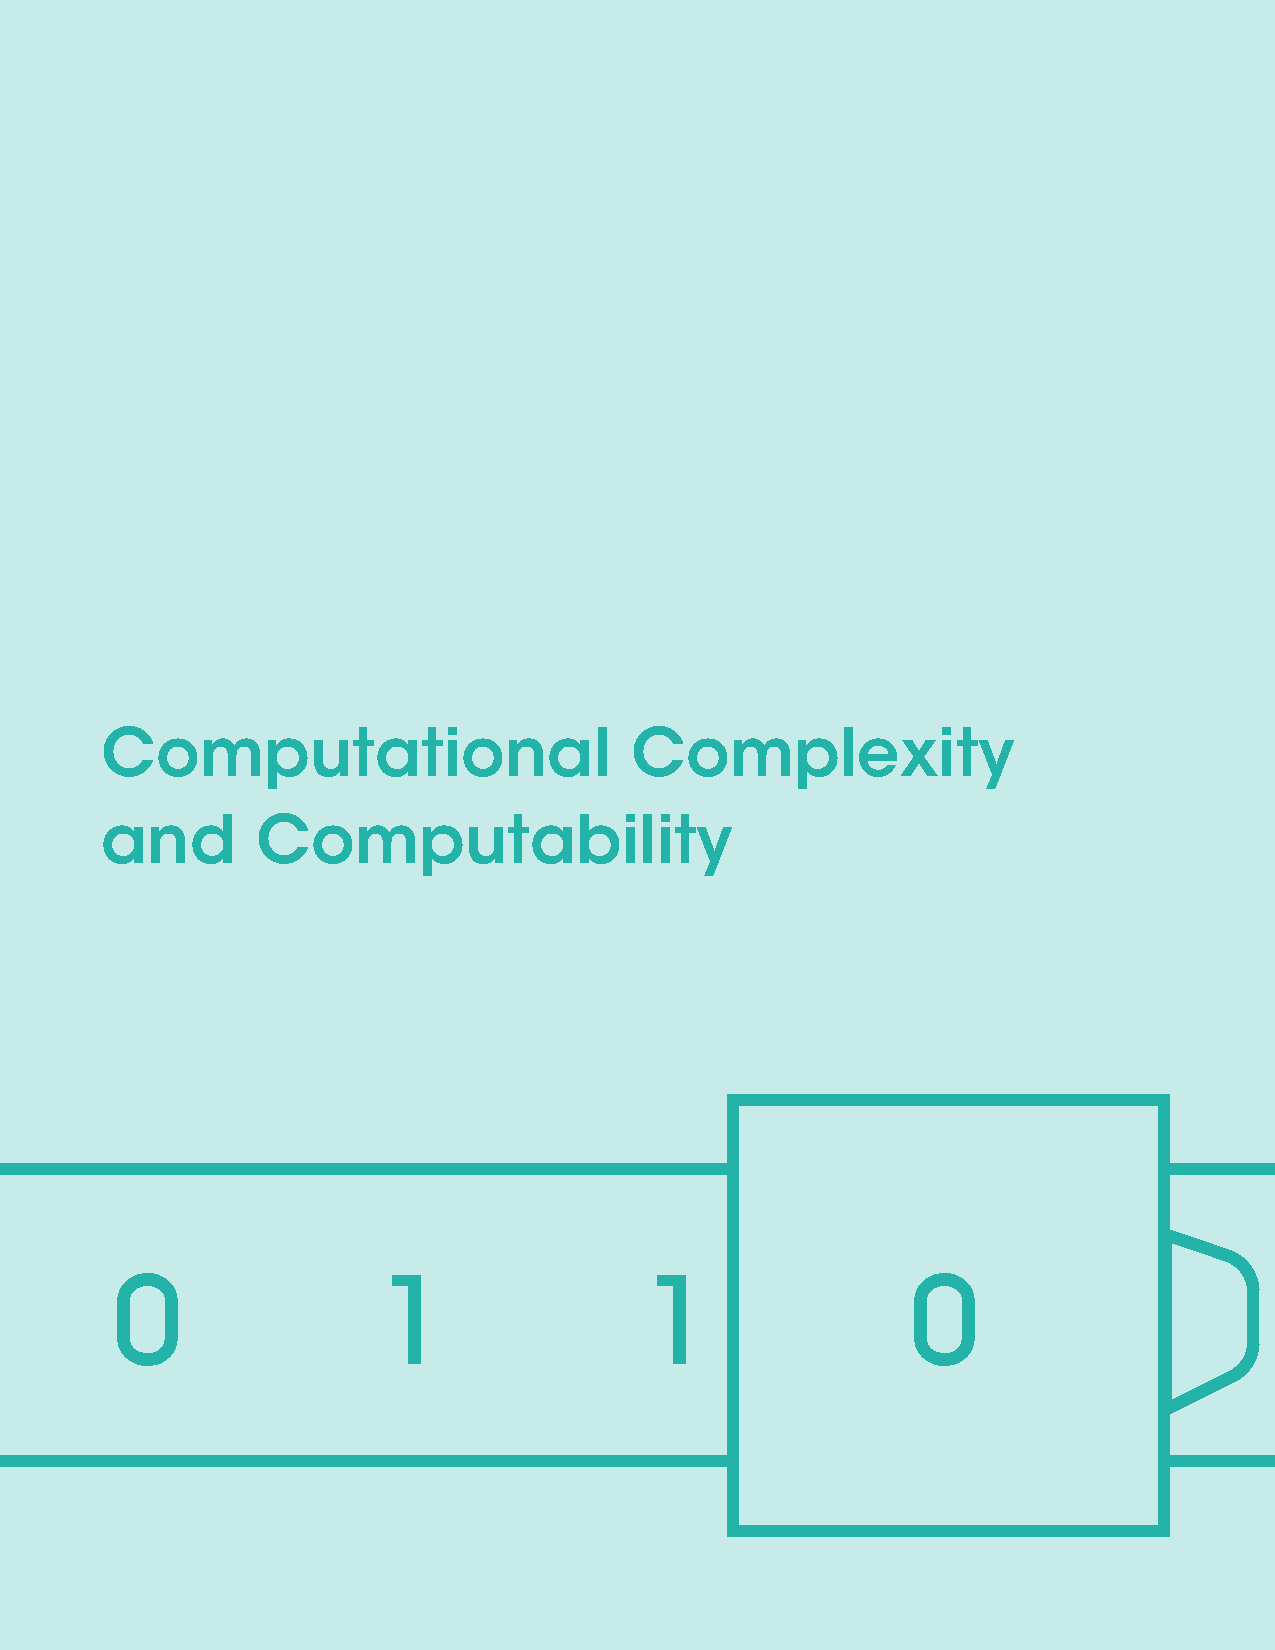
\includepdf[pages=-]{complexity_cover.pdf}

%----------------------------------------------------------------------------------------
%	COPYRIGHT PAGE
%----------------------------------------------------------------------------------------

\newpage
The cover depicts a Turing machine. Turing machine is a simple but powerful computation model used to study the computability and complexity of problems. It is considered one of the foundational models of theoretical computer science.
~\vfill
\thispagestyle{empty}

\noindent Copyright \copyright\ \the\year{} Kevin Gao % Copyright notice

\hfill

\noindent \textsc{terra-incognita.dev} % URL

\hfill

% License information
\noindent Licensed under the Creative Commons Attribution-NonCommercial 3.0 Unported License (the ``License''). You may not use this file except in compliance with the License. You may obtain a copy of the License at \url{http://creativecommons.org/licenses/by-nc/3.0}. Unless required by applicable law or agreed to in writing, software distributed under the License is distributed on an \textsc{``as is'' basis, without warranties or conditions of any kind}, either express or implied. See the License for the specific language governing permissions and limitations under the License.


%----------------------------------------------------------------------------------------
%	TABLE OF CONTENTS
%----------------------------------------------------------------------------------------

%\usechapterimagefalse % If you don't want to include a chapter image, use this to toggle images off - it can be enabled later with \usechapterimagetrue

 % Table of contents heading image

\pagestyle{empty} % Disable headers and footers for the following pages
\usechapterimagefalse
\tableofcontents % Print the table of contents itself

\cleardoublepage % Forces the first chapter to start on an odd page so it's on the right side of the book

\pagestyle{fancy} % Enable headers and footers again

%----------------------------------------------------------------------------------------
%	PART
%----------------------------------------------------------------------------------------
\setlength{\parskip}{1em}

\part{Automata and Languages}

\chapter{Regular Language}
\section{Alphabet and Strings}

$\Sigma$ denotes a finite alphabet of symbols. $\Sigma^*$ denotes a set of all strings, including the empty string $\epsilon$, consist of elements of $\Sigma$.

For string $x \in \Sigma^*$, $|x|$ is the length of $x$. A language is a subset of $\Sigma^*$.

\section{Regular Language}

See 240 notes.

Example: $\\mathrm{Even} = \{ w \in \{0,1\}^* \mid \text{$w$ contains an even number of 1's}\}$. It can be expressed using the regular expression $0^* + (0^*10^*10^*)^*$.

It also has a 2-state deterministic finite automaton that decides the language $\mathsf{Even}$.
\begin{center}
    \begin{tikzpicture}
    \node[state,initial,accepting] (qeven) {\( q_{even} \)};
    \node[state] (qodd) [right=of qeven] {\( q_{odd} \)};
    \path[->] (qeven) edge [above,bend left=20] node {1} (qodd);
    \path[->] (qodd) edge [below,bend left=20] node {1} (qeven);
    \path[->] (qeven) edge [loop above] node {0} (qeven);
    \path[->] (qodd) edge [loop above] node {0} (qodd);
    \end{tikzpicture}
\end{center}

More formally,
\begin{definition}[Deterministic Finite State Automata]
    A deterministic finite state automaton (DFA) is a quintuple (5-tuple)
    $$
    M = (Q,\Sigma,\delta,s,F)
    $$
    where
    \begin{itemize}
        \item $Q$ is a finite set of states
        \item $\Sigma$ is a finite set called the alphabet
        \item $\delta:\, Q\times\Sigma \to Q$, the transition function
        \item $s \in Q$, the starting state
        \item $F \subseteq Q$, the set of accepting states
    \end{itemize}
\end{definition}

\chapter{Context-Free Language}
\input{notes/cfl.tex}

\chapter{Turing Machine}
\section{Turing Machine}

While finite state automata and pushdown automata are all valid models of computation, they are too restricted as models of general purpose computers. Our goal is to have a model so that we can define computation as abstractly and general as possible.

How do we define algorithms rigorously? What does it mean for an algorithm to run in polynomial time. How do we argue that efficient algorithms do not exist.

Turing machine is a model of computation first proposed by Alan Turing in 1936. It is much more powerful than previous models that we have looked at. It is sufficiently general and can model what a human can do. A Turing machine can be think of a finite automata with unlimited and unrestricted memory.

In a Turing machine, we have an \textbf{one-way infinite tape} divided into ``cells'', each holding one symbol, including the blank symbol $\sqcup$. It also has a \textbf{read-write} head positioned in one square at a time that can move to the left or right. The control of the Turing is in of a fixed number of states. (The blank symbol $\sqcup$ is sometimes denoted by $\not b$ or $\square$ )

Initially, the input tape contains a finite number of symbols starting at the left-most cell with the remaining cells blank. The head starts at the left-most input symbol. Current state and symbol determine the next state, symbol written, and the movement of the head (either one square left or one square right).

\begin{figure}[htbp]
    \centering
    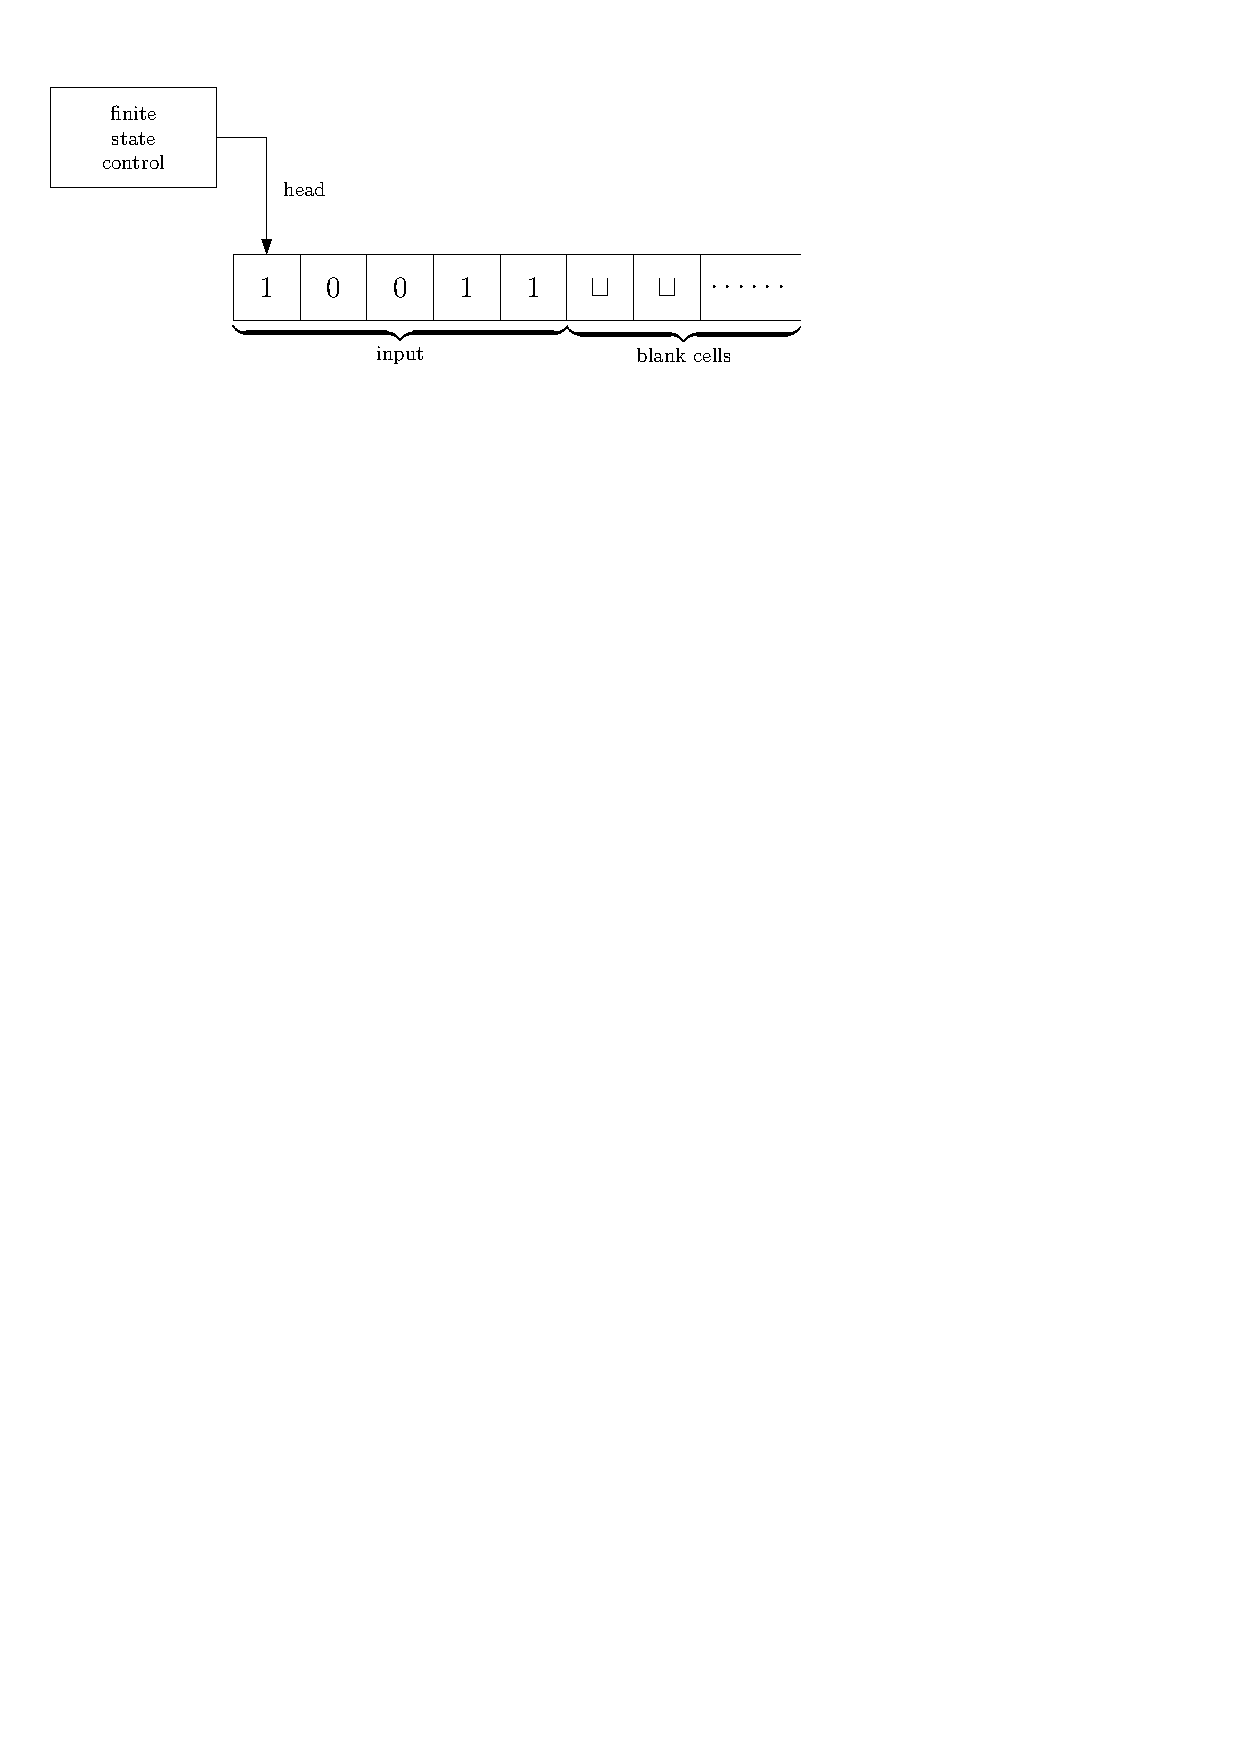
\includegraphics[width=0.7\linewidth]{tm.pdf}
    \caption{A Turing machine}
    \label{fig:tm}
\end{figure}

\begin{definition}[Turing Machine]
    A Turing machine is a 7-tuple $(Q,\Sigma,\Gamma,\delta,q_0,q_{accept},q_{reject})$ where $Q,\Sigma,\Gamma$ are all finite sets, and
    \begin{itemize}
        \item $Q$ is the set of states
        \item $\Sigma$ is the input alphabet not containing the blank symbol $\sqcup$
        \item $\Gamma$ is the tape alphabet, where $\sqcup \in \Gamma$ and $\Sigma \subset \Gamma$
        \item $\delta:\;(Q-\{q_{accept},q_{reject}\}) \times \Gamma \to Q \times \Gamma \times \{L,R\}$ is the transition function
        \item $q_0 \in Q$ is the start state
        \item $q_{accept} \in Q$ is the accept state
        \item $q_{reject} \in Q$ is the reject state, where $q_{accept} \neq q_{reject}$ 
    \end{itemize}
\end{definition}

$\delta(q,a) = (q',a',x)$ where $x \in \{L,R\}$ means if a machine is in state $q$ and head positioned on a square containing $a$, then the machine replaces $a$ with $a'$, moves to state $q$, and moves the head left ($L$) or right ($R$) depending on the direction given by $x$.

A Turing machine $M$ works as follows on input string $x \in \Sigma^*$.
\begin{enumerate}
    \item Initially $x = x_1x_2\ldots x_n \in \Sigma^*$ appears on leftmost $n$ squares of the input tape. Rest of the tape is blank;
    \item Head of $M$ starts on the leftmost square of tape;
    \item Initial state is $q_0$ 
    \item $M$ moves according to the transition function $\delta$
    \item Continue until $M$ reaches $q_{accept}$ or $q_{reject}$ and then $M$ halts. Otherwise, continue on forever.
\end{enumerate}

\begin{definition}[Language Recognized by Turing Machine]
    We say a Turing machine $M$ \textbf{accepts} a string $x \in \Sigma^*$ if $M$ upon reading the input $x$ eventually \textbf{halts} in state $q_{accept}$.

    Let $L(M) = \{x \in \Sigma^* \mid \text{$M$ accepts $x$} \}$. We say $L(M)$ is the \textbf{language recognized/accepted by} $M$. We say $x \not\in L(M)$ if $M$ upon reading $x$ either \textbf{halts} in $q_{reject}$ or \textbf{loops}.
\end{definition}

\begin{example}[Palindrome]
    $$\mathrm{Palindrome} = \{yy^R \mid y \in \{0,1\}^*\}$$
    At a high level, the \textbf{Turing machine} that decides this language scans back and forth, matching and erasing leftmost and rightmost symbols. Accept if the input is completely earased or reject if otherwise.
\end{example}

\section{Configuration of Turing Machine}

The \textbf{configuration} of a Turing machine describes the state, head position, and tape contents. It is denoted $x q y$ where $x,y \in \Gamma^*$ and $q \in  Q$. In this notation, the head position is implied to be the leftmost symbol of $y$.

Note that $xqy$ and $xqy \sqcup$ are equivalent configurations, but $xqy$ and $\sqcup xqy$ are not equivalent. Whether or not the first symbol is blank is important.

\begin{definition}
    Given two configurations $C_1$ and $C_2$, we say configuration $C_1$ \textbf{yields} $C_2$ if $C_2$ follows from $C_1$ by one step of $M$ (one application of $\delta$).
\end{definition}

\begin{example}
    Let $x,y \in \Gamma^*$ and $a,b \in \Gamma$. If $\delta(q,a) = (q',a',R)$, then $xqay$ yields $xa'q'y$. If $\delta(q,b) = (q',b',L)$, then $xaqby$ yields $xq'ab'y$. $qby$ yields $q'b'y$ because the tape head cannot move left anymore.
\end{example}

\begin{definition}[Computation]
    The \textbf{computation} of $M$ on input $x \in \Sigma^*$ is the sequence $C_0C_1C_2\ldots$ where $C_0 = q_0x$ and each configuration follows from the previous one. We say the computation is \textbf{halting} if it eventually reaches accept or reject state. Otherwise, we say the computation is \textbf{looping} (infinite).
\end{definition}

\section{Decidability and Recognizability}

\begin{definition}[Decider]
    A Turing machine $M$ is a decider if it halts on all inputs $x \in \Sigma^*$.
\end{definition}

\begin{definition}[Turing Decidable and Turing Recognizable]
    A language $A \in \Sigma^*$ is Turing decidable if and only if there is a \textbf{decider} $M$ such that $L(M)=A$.

    $A$ is semidecidable/Turing recognizable if and only if there is a Turing machine $M$ such that $L(M)=A$. In this case, $M$ may not halt if it does not accept $A$ (reject by looping).
\end{definition}

\section{Some Classes of Languages}

$\textsf{D} = \{ A \subseteq \Sigma^* \mid \text{$A$ is decidable}$

$\textsf{SD} = \{A \subseteq \Sigma^* \mid \text{$A$ is semidecidable}$

$\textsf{P} = \{A \subseteq \Sigma^* \mid \text{$A=L(M)$ for some $M$ that halts in polynomial time} \}$

Later, we will show that $\textsf{P} \subsetneq \textsf{D} \subsetneq \textsf{SD}$.

\section{Difference Between FSA and TM}

\begin{itemize}
    \item TM can read and write symbols. Infinite tape.
    \item Head can move left or right, unless the head is at left-most position.
    \item Special ``accept'' and ``reject'' states that stop computation immediately. The machine halts only when it reaches an accept or reject state. On the other hand, an FSA can only perform a finite amount of transitions before it halts.
\end{itemize}

\part{Decidability and Computability}

\chapter{Undecidable Language}
\section{Countability}

\vspace{\parskip}

\begin{definition}[Countable Set]
    A set $A$ is countable if $A$ is empty or there is a injective function $f:\, A \to \N$, or equivalently, a surjective function $f:\, \N \to A$.
\end{definition}

\begin{theorem}
    $\R$ is not countable.
\end{theorem}

\begin{theorem}
    $2^{\N} = \mathcal{P}(\N)$ is not countable.
\end{theorem}

\begin{corollary}
    There exists some $A \subseteq \Sigma^*$ such that $A$ is not Turing-recognizable.
\end{corollary}

\begin{proof}
    We will prove this by showing that the set of all languages in $\Sigma^*$ is not countable, but the set of Turing-recognizable languages is countable.

    We first show that $\Sigma^*$ is countable. To show this, we simply list all strings in $\Sigma^*$ in lexicographic order.

    Observe that $\mathsf{TR} = \{ A \subseteq \Sigma^* \mid A = L(M) \}$ is also countable because the number of Turing machines is countable, each of which can be encoded as a finite length string.

    But the set of all languages $\{ A \subseteq \Sigma^* \} = 2^{\Sigma^*}$. By Cantor's theorem, since $\Sigma^*$ is countably infinite, the power set of $\Sigma^*$ is uncountable.

    Hence, there exists some language $A \subseteq \Sigma^*$ that is not Turing-recognizable.
\end{proof}

Let $\langle M \rangle$ denote the encoding of a Turing machine $M$. For $n \in \N$, let $\langle n \rangle \in \{0,1\}^*$ be the binary encoding of $n$. For a sequence of numbers $n_1,n_2,\ldots,n_k$, $\langle n_1,n_2,\ldots,n_k \rangle \in \{0,1,\#\}^*$ be $\langle n_1 \rangle \# \langle n_2 \rangle \# \cdots \# \langle n_k \rangle$.

Then, any Turing machine can be determined by a finite sequence of numbers specifying $|Q|$, $|\Sigma|$, $|\Gamma|$, identity of $q_0,q_{accept},q_{reject}$, and a sequence of numbers specifying $\delta$.

$$
\langle M \rangle = \text{the string that determines $M$}
$$

Furthermore, we can denote a Turing machine $T$ with input $w$ as $\langle M, w \rangle$.

\begin{theorem}
    Let
    $$
    \mathsf{DIAG} = \{ \langle M \rangle \mid \text{$M$ is a TM and $\langle M \rangle \not\in L(M)$} \}
    $$
    $\mathsf{DIAG}$ is not Turing recognizable.
\end{theorem}

\begin{proof}
    Suppose, for contradiction, that there exists a TM $M$ such that $T(M) = \mathsf{DIAG}$. Then, we can ask if $\langle M \rangle \in L(M)$.

    Suppose that $\langle M \rangle \in L(M)$. Then
    $$
    \langle M \rangle \in L(M) \iff \langle M \rangle \in \mathsf{DIAG} \iff \langle M \rangle \not\in \in L(M)
    $$
    which is a contradiction.
\end{proof}

This is similar to Russell's paradox.

\begin{theorem}
    Every finite language is Turing recognizable and decidable.
\end{theorem}

\begin{theorem}
    Every regular language is Turing recognizable and decidable.
\end{theorem}

\section{Universal Turing Machine}

Let $A_{\mathsf{TM}}$ be the language
$$
\{ \langle M,w \rangle \mid \text{$M$ accepts $w$} \}
$$

\begin{theorem}
    $A_{\mathsf{TM}}$ is Turing-recognizable.
\end{theorem}

\begin{proof}
    We show that there exists a TM $U$ such that $L(U) = A_{\mathsf{TM}}$. $U$ decodes $\langle M \rangle$ into a TM $M$ and simulates $M$ on $w$. Thus, $A_{\mathsf{TM}}$ is Turing-recognizable.
\end{proof}

The $U$ that we have constructed to recognize $A_{\mathsf{TM}}$ is called a universal Turing machine.

\begin{theorem}
    $A_{\mathsf{TM}}$ is not decidable.
\end{theorem}

%----------------------------------------------------------------------------------------
%	APPENDIX
%----------------------------------------------------------------------------------------
\part*{Appendix}
\appendix
\chapter*{Commonly Used Axioms \& Theorems}
\addcontentsline{toc}{chapter}{\textcolor{ocre}{Axioms \& Theorems}} 

\renewcommand{\leftmark}{\sffamily\bfseries Axioms \& Theorems}
\renewcommand{\rightmark}{\sffamily\bfseries Axioms \& Theorems}

\section*{Rules of Inference} \label{rulesofinference}

\begin{axiom_appendix}[Modus Ponens]
$(P \wedge (P \implies Q)) \implies Q $
\end{axiom_appendix}

\begin{axiom_appendix}[Modus Tollens]
$(\neg Q \wedge (P \implies Q)) \implies \neg P $
\end{axiom_appendix}

\begin{axiom_appendix}[Hypothetical Syllogism (transitivity)]
\hfill

$((P \implies Q) \wedge (Q \implies R)) \implies (P \implies R) $
\end{axiom_appendix}

\begin{axiom_appendix}[Disjunctive Syllogism]
$((P \vee Q) \wedge \neg P) \implies Q$
\end{axiom_appendix}

\begin{axiom_appendix}[Addition]
$P \implies (P \vee Q)$
\end{axiom_appendix}

\begin{axiom_appendix}[Simplification]
$(P \wedge Q) \implies P$
\end{axiom_appendix}

\begin{axiom_appendix}[Conjunction]
$((P) \wedge (Q)) \implies (P \wedge Q)$
\end{axiom_appendix}

\begin{axiom_appendix}[Resolution]
$((P \vee Q) \wedge (\neg P \vee R)) \implies (Q \vee R)$
\end{axiom_appendix}

\section*{Laws of Logic}

\begin{axiom_appendix}[Implication Law]
$(P \implies Q) \equiv (\neg P \vee Q)$
\end{axiom_appendix}

\begin{axiom_appendix}[Distributive Law]
\begin{align*}
    (P \wedge (Q \vee R)) &\equiv ((P \wedge Q) \vee (P \wedge R)) \\
    (P \vee (Q \wedge R)) &\equiv ((P \vee Q) \wedge (P \vee R))
\end{align*}
\end{axiom_appendix}

\begin{axiom_appendix}[De Morgan's Law]
\begin{align*}
    \neg (P \wedge Q) &\equiv (\neg P \vee \neg Q) \\
    \neg (P \vee Q) &\equiv (\neg P \wedge \neg Q)
\end{align*}
\end{axiom_appendix}

\begin{axiom_appendix}[Absorption Law]
\begin{align*}
    (P \vee (P \wedge Q)) &\equiv P \\
    (P \wedge (P \vee Q)) &\equiv P
\end{align*}
\end{axiom_appendix}

\begin{axiom_appendix}[Commutativity of AND]
$A \wedge B \equiv B \wedge A$
\end{axiom_appendix}

\begin{axiom_appendix}[Associativity of AND]
$(A \wedge B) \wedge C \equiv A \wedge (B \wedge C)$
\end{axiom_appendix}

\begin{axiom_appendix}[Identity of AND]
$\textbf{T} \wedge A \equiv A$
\end{axiom_appendix}

\begin{axiom_appendix}[Zero of AND]
$\textbf{F} \wedge A \equiv \textbf{F}$
\end{axiom_appendix}

\begin{axiom_appendix}[Idempotence for AND]
$A \wedge A \equiv A$
\end{axiom_appendix}

\begin{axiom_appendix}[Contradiction for AND]
$A \wedge \neg A \equiv \textbf{F}$
\end{axiom_appendix}

\begin{axiom_appendix}[Double Negation]
$\neg (\neg A) \equiv A$
\end{axiom_appendix}

\begin{axiom_appendix}[Validity for OR]
$A \vee \neg A \equiv \textbf{T}$
\end{axiom_appendix}

\section*{Induction}

\vspace{\parskip}

\begin{axiom_appendix}[Well Ordering Principle]
Every nonempty set of nonnegative integers has a smallest element. i.e., For any $A \subset \N$ such that $A \neq \emptyset$, there is some $a \in A$ such that $\forall a' \in A.a\leq a'$.
\end{axiom_appendix}

\section*{Recurrences}

\vspace{\parskip}

\begin{theorem_appendix}[The Master Theorem]
Suppose that for $n \in \Z^+$.
\begin{equation*}
    T(n) =
    \begin{cases}
    c & \text{if $n<B$} \\
    a_1 T(\lceil n/b \rceil) + a_2 T(\lfloor n/b \rfloor) + dn^i & \text{if $n\geq B$}
    \end{cases}
\end{equation*}
where $a_1, a_2, B, b \in \N$.

Let $a = a_1+a_2 \geq 1$, $b>1$, and $c,d,i \in \R \cup \{0\}$. Then,
\begin{equation*}
    T(n) \in
    \begin{cases}
    O(n^i \log n) & \text{if $a=b^i$} \\
    O(n^i) & \text{if $a < b^i$} \\
    O(n^{\log_b a}) & \text{if $a > b^i$}
    \end{cases}
\end{equation*}
\end{theorem_appendix}

Linear Recurrences:

A linear recurrence is an equation
$$
f(n) = \underbrace{a_1 f(n-1) + a_2 f(n-2) + \cdots + a_d f(n-d)}_{\text{homogeneous part}}  + \underbrace{g(n)}_{\text{inhomogeneous part}}
$$
along with some boundary conditions.

The procedure for solving linear recurrences are as follows:

\begin{enumerate}
    \item Find the roots of the characteristic equation. Linear recurrences usually have exponential solutions (such as $x^n$). Such solution is called the \textbf{homogeneous solution}.
    $$
    x^n = a_1 x^{n-1} + a_2 x^{n-2} + \cdots + a_{k-1} x + a_k
    $$
    \item Write down the homogeneous solution. Each root generates one term and the homogeneous solution is their sum. A non-repeated root $r$ generates the term $cr^n$, where $c$ is a constant to be determined later. A root with $r$ with multiplicity $k$ generates the terms
    $$
    d_1r^n \quad d_2nr^n \quad d_3n^2r^n \quad \cdots \quad d_kn^{k-1}r^n
    $$
    where $d_1,\cdots,d_k$ are constants to be determined later.
    \item Find a \textbf{particular solution} for the full recurrence including the inhomogeneous part, but without considering the boundary conditions.
    
    If $g(n)$ is a constant or a polynomial, try a polynomial of the same degree, then of one higher degree, then two higher. If $g(n)$ is exponential in the form $g(n) = k^n$, then try $f(n) = ck^n$, then $f(n) = (bn+c)k^n$, then $f(n) = (an^2+bn+c)k^n$, etc.
    
    \item Write the \textbf{general solution}, which is the sum of homogeneous solution and particular solution.
    \item Substitute the boundary condition into the general solution. Each boundary condition gives a linear equation. Solve such system of linear equations for the values of the constants to make the solution consistent with the boundary conditions.
\end{enumerate}


\chapter*{Basic Prerequisite Mathematics}
\addcontentsline{toc}{chapter}{\textcolor{ocre}{Basic Prerequisite Mathematics}}
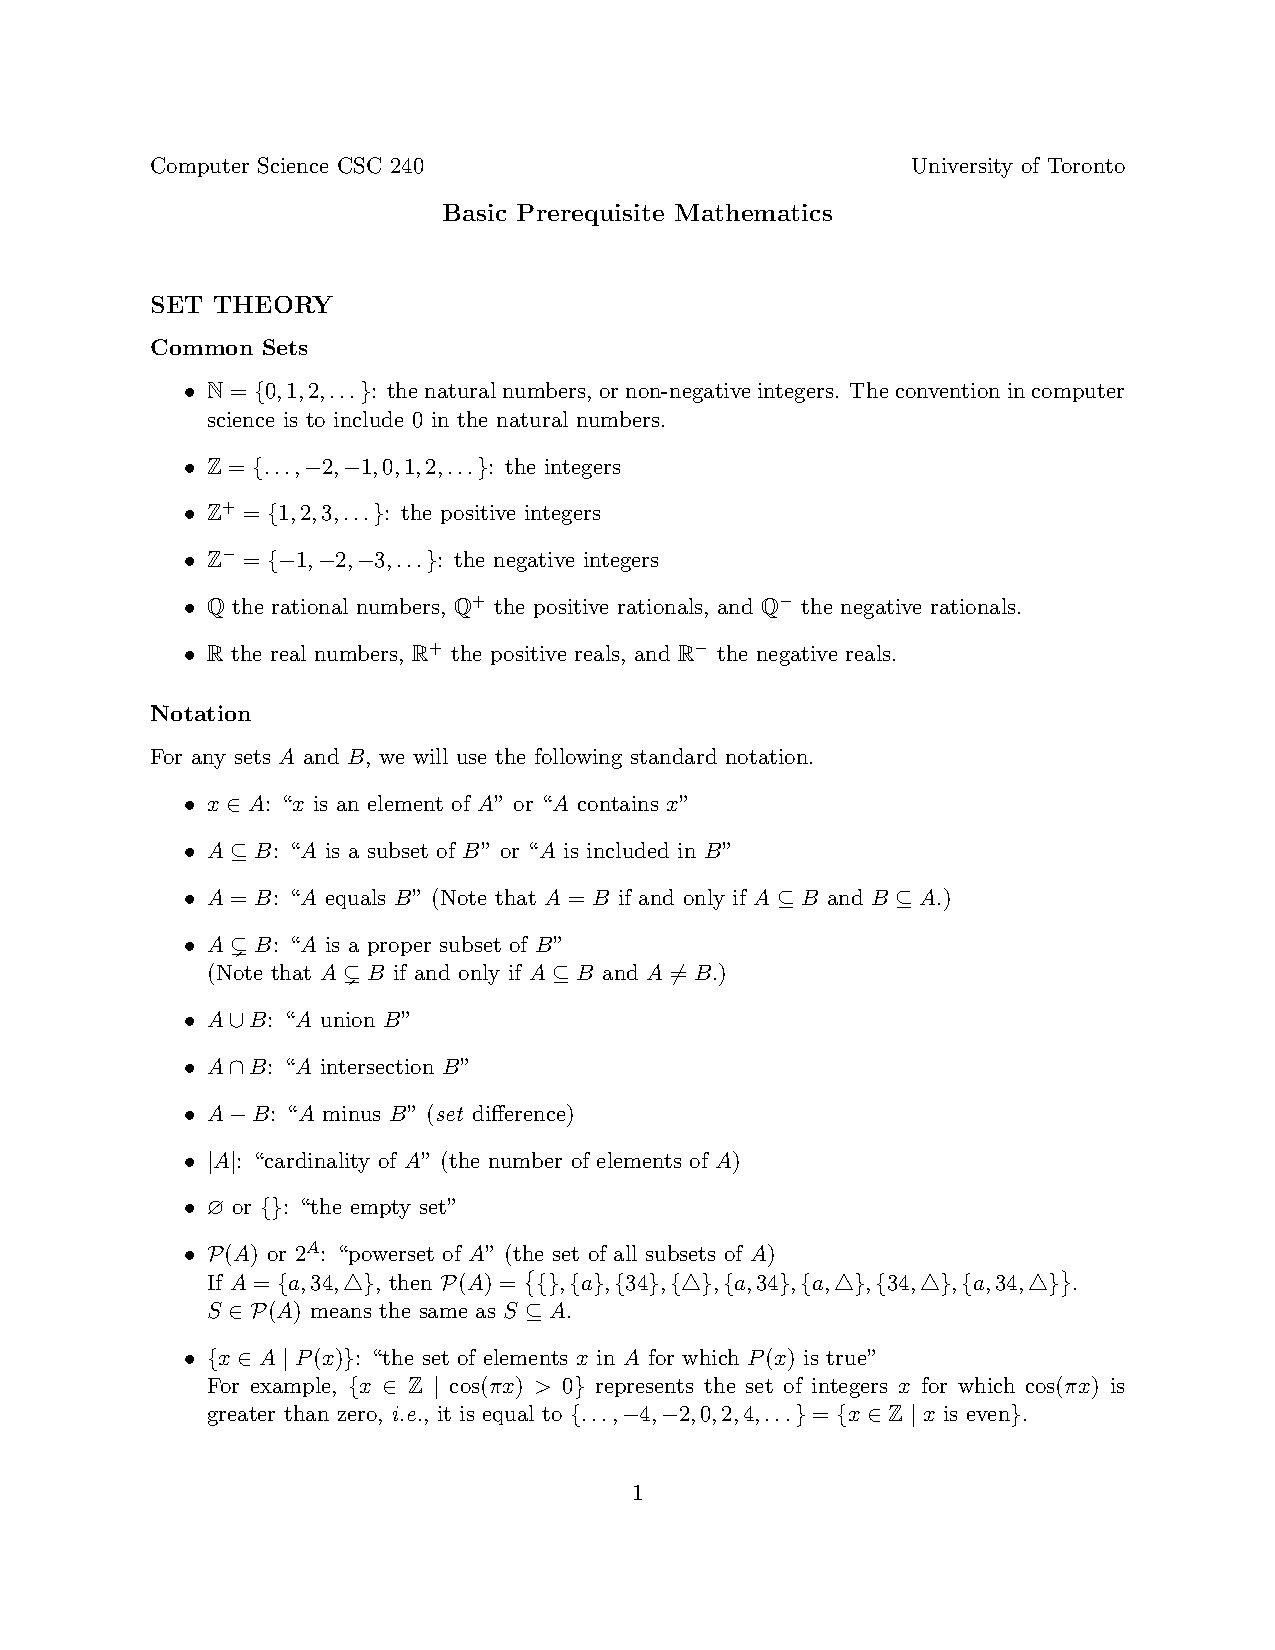
\includepdf[pages=-]{appendix/basicMath.pdf}

\chapter*{Proof Templates}
\addcontentsline{toc}{chapter}{\textcolor{ocre}{Proof Templates}}
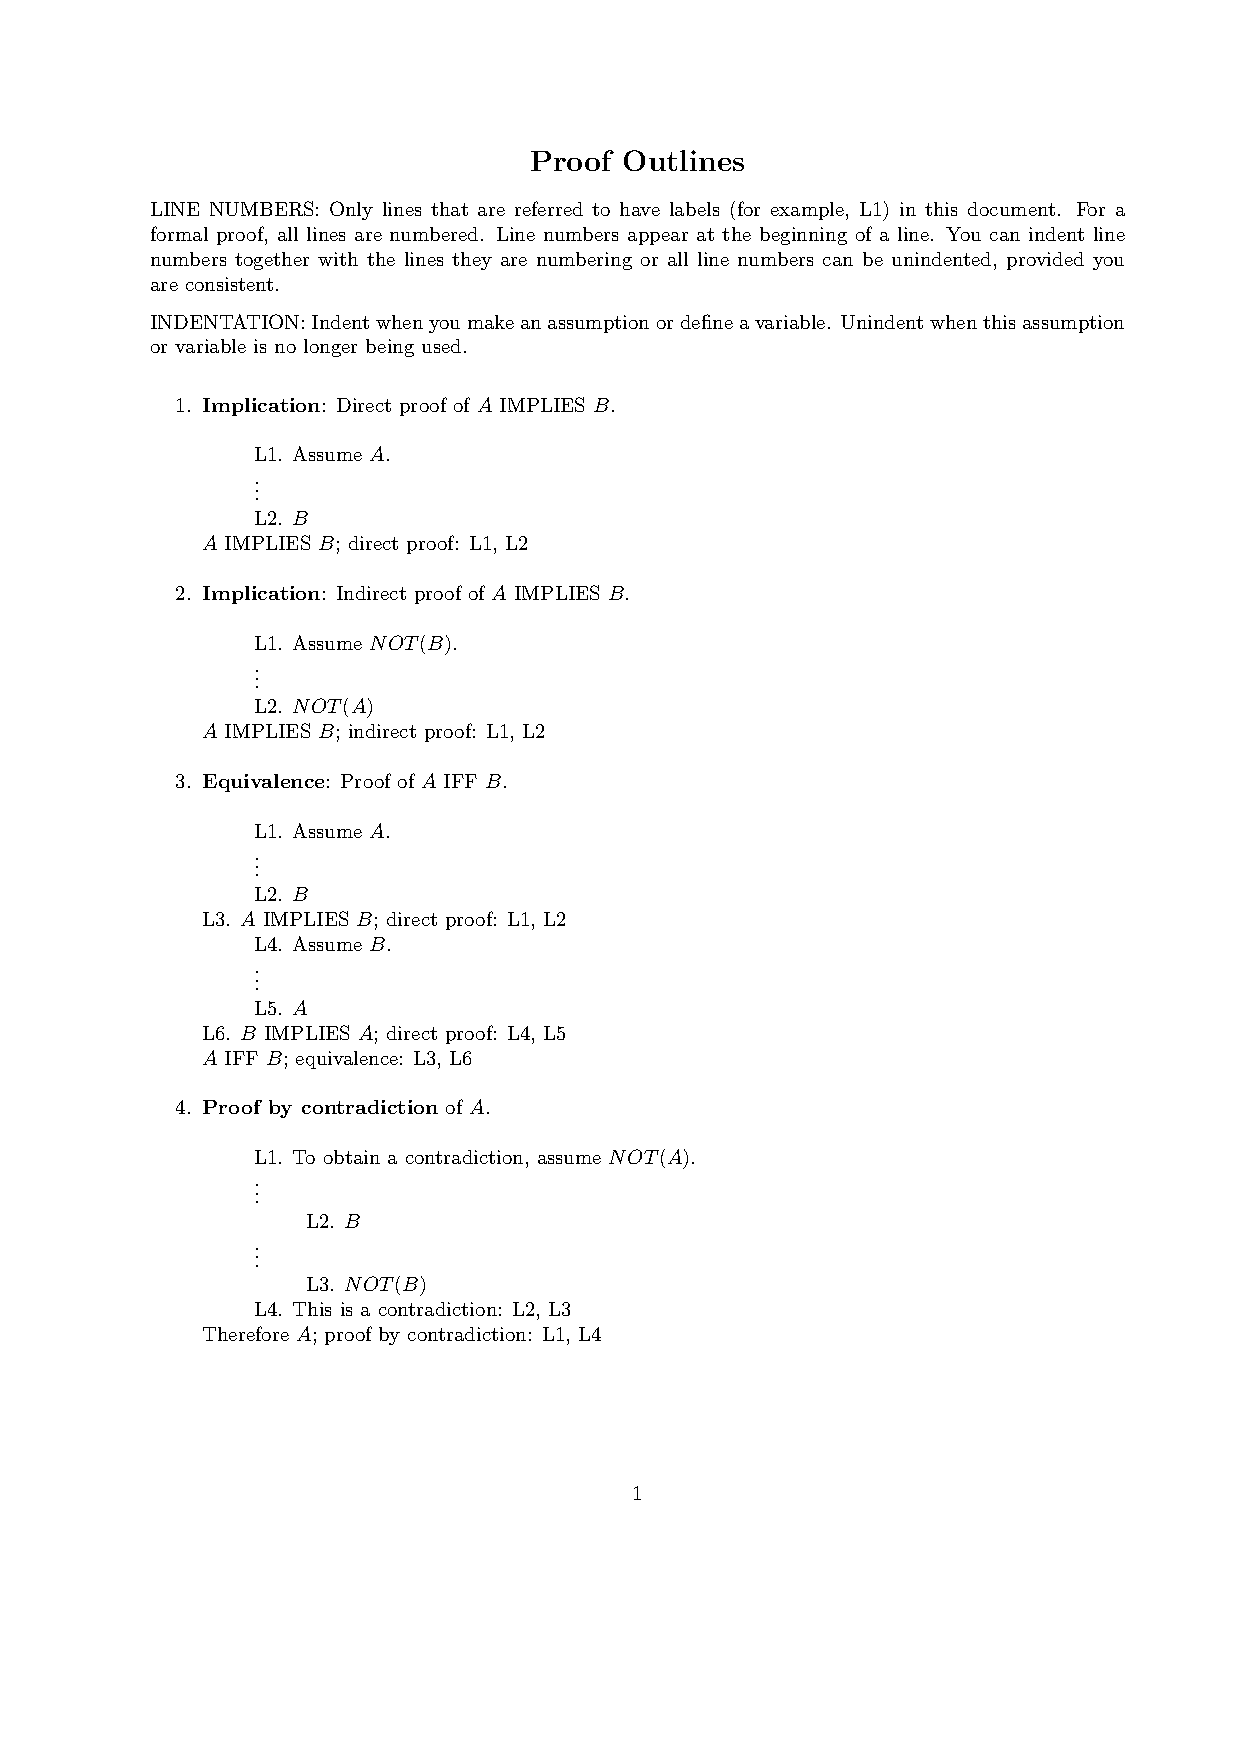
\includepdf[pages=-]{appendix/proofOutlines.pdf}

%----------------------------------------------------------------------------------------
%	INDEX
%----------------------------------------------------------------------------------------

\chapter*{Index}
\renewcommand{\leftmark}{\sffamily\bfseries Index}
\renewcommand{\rightmark}{\sffamily\bfseries Index}
%\cleardoublepage % Make sure the index starts on an odd (right side) page
\setlength{\columnsep}{0.75cm} % Space between the 2 columns of the index
\addcontentsline{toc}{chapter}{\textcolor{ocre}{Index}} % Add an Index heading to the table of contents

\printindex % Output the index

%------------------------------------------------
%   BIBLIOGRAPHY ENTRIES
%------------------------------------------------
\chapter*{Bibliography}
\renewcommand{\leftmark}{\sffamily\bfseries Bibliography}
\renewcommand{\rightmark}{\sffamily\bfseries Bibliography}
\addcontentsline{toc}{chapter}{\textcolor{ocre}{Bibliography}} % Add a Bibliography heading to the table of contents

\section*{Courses}
\addcontentsline{toc}{section}{Courses}
\printbibliography[heading=bibempty,type=misc]

\section*{Books}
\addcontentsline{toc}{section}{Books}
\printbibliography[heading=bibempty,type=book]

\section*{Journal Articles}
\addcontentsline{toc}{section}{Journal Articles}
\printbibliography[heading=bibempty,type=article]

\newpage

%------------------------------------------------
%   TUTORIALS
%------------------------------------------------

%----------------------------------------------------------------------------------------

\end{document}
